\documentclass[aspectratio=169]{beamer}
\usetheme{TUDelft}

% Packages
\usepackage{amsmath}
\usepackage{amssymb}
\usepackage{algorithm}
\usepackage{algorithmic}
\usepackage{graphicx}
\usepackage{tikz}
\usepackage{booktabs}
\usepackage{listings}
\usepackage{xcolor}
\usepackage{pifont}

% Python code styling
\lstset{
    language=Python,
    basicstyle=\ttfamily\footnotesize,
    keywordstyle=\color{blue},
    commentstyle=\color{gray},
    stringstyle=\color{red},
    showstringspaces=false,
    breaklines=true,
    frame=single,
    numbers=left,
    numberstyle=\tiny\color{gray}
}

% TikZ libraries
\usetikzlibrary{shapes,arrows,positioning,calc}

% Title information
\title[Learning to Rank]{Lecture 6: Learning to Rank}
\subtitle{The Machine Learning Framework for IR}
\author{Avishek Anand}
\institute{Information Retrieval}
\date{\today}

\begin{document}

% Title slide
\begin{frame}
\titlepage
\end{frame}

% Course Context


% Outline
\begin{frame}{Outline}
\tableofcontents
\end{frame}

% ====================================================================
% SECTION 1: LTR BASICS
% ====================================================================
\section{Intro to Learning to Rank (LTR)}

\begin{frame}{The Motivation for LTR}
\begin{itemize}
    \item We have many signals: BM25, PageRank, Recency, Neural Score, Hybrid score...
    \item \textbf{Manually tuning} weights ($\lambda_1, \lambda_2, \dots$) is impossible.
    \item \textbf{Solution:} Treat ranking as a supervised machine learning problem.
\end{itemize}

\vspace{1em}
\begin{block}{Input Features for $(q, d)$}
\begin{itemize}
    \item \textbf{Query-independent:} PageRank, document length.
    \item \textbf{Query-dependent:} BM25, TF-IDF, BERT similarity.
    \item \textbf{User-dependent:} Search history, localization.
\end{itemize}
\end{block}
\end{frame}

% ====================================================================
% SECTION 2: POINTWISE, PAIRWISE, LISTWISE
% ====================================================================
\section{Pointwise, Pairwise, Listwise}

\begin{frame}{Three Approaches to LTR}
\begin{columns}
\begin{column}{0.31\textwidth}
\textbf{Pointwise}
\begin{itemize}
    \item Predict score for a \textbf{single} doc.
    \item Regression/Classification.
    \item Ignores relative order.
\end{itemize}
\end{column}

\begin{column}{0.31\textwidth}
\textbf{Pairwise}
\begin{itemize}
    \item Predict relative order of a \textbf{pair} $(d_1, d_2)$.
    \item Minimize misordered pairs.
    \item \textit{Example: RankNet, LambdaRank.}
\end{itemize}
\end{column}

\begin{column}{0.31\textwidth}
\textbf{Listwise}
\begin{itemize}
    \item Optimize the \textbf{entire} list.
    \item Directly optimize NDCG or MAP.
    \item \textit{Example: LambdaMART.}
\end{itemize}
\end{column}
\end{columns}
\end{frame}

\begin{frame}{The LambdaMART Logic}
\begin{itemize}
    \item MART (Multiple Additive Regression Trees) = \textbf{Gradient Boosting}.
    \item IR metrics (NDCG) are discrete (not differentiable).
    \item \textbf{Trick:} Use "Lambda" gradients that approximate the change in NDCG caused by swapping two docs.
\end{itemize}

\vspace{1em}
\begin{center}
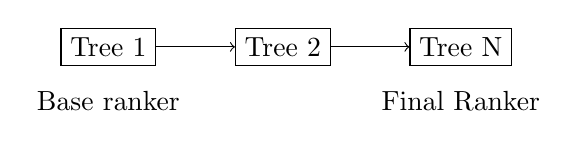
\begin{tikzpicture}
    \node[draw, rectangle] (t1) {Tree 1};
    \node[draw, rectangle, right=1cm of t1] (t2) {Tree 2};
    \node[draw, rectangle, right=1cm of t2] (tn) {Tree N};
    
    \draw[->] (t1) -- (t2);
    \draw[->] (t2) -- (tn);
    
    \node[below=0.2cm of t1] {Base ranker};
    \node[below=0.2cm of tn] {Final Ranker};
\end{tikzpicture}
\end{center}
\end{frame}

% ====================================================================
% SECTION 3: EVALUATION METRICS
) % ====================================================================
\section{Evaluation Metrics: Beyond Precision}

\begin{frame}{Normalized Discounted Cumulative Gain (NDCG)}
\textbf{Concept:} Reward relevant documents in rank position $i$, but discount them as $i$ increases.

\vspace{1em}
\begin{block}{Formula}
$$\text{DCG}_p = \sum_{i=1}^p \frac{2^{rel_i} - 1}{\log_2(i+1)}, \quad \text{NDCG}_p = \frac{\text{DCG}_p}{\text{IDCG}_p}$$
\end{block}

\vspace{1em}
\begin{itemize}
    \item $rel_i$: Relevance grade (0, 1, 2, 3).
    \item IDCG: "Ideal" DCG (sorted by relevance).
    \item \textbf{Why use it?} Accounts for graded relevance and position.
\end{itemize}
\end{frame}

% ====================================================================
% SUMMARY
% ====================================================================
\section{Final Course Summary}

\begin{frame}{The Complete IR Journey}
\begin{itemize}
    \item \textbf{Foundations:} Boolean Retrieval and the Vector Space Model.
    \item \textbf{Engineering:} Efficient Indexing and Compression.
    \item \textbf{Queries:} Query Understanding and Evaluation.
    \item \textbf{Classical Ranking:} BM25 and Language Modeling.
    \item \textbf{Neural Shift:} Embeddings, Transformers, and Re-ranking.
    \item \textbf{Modern Search:} Full-corpus Dense Retrieval (DPR).
    \item \textbf{Application:} Recommender Systems and RAG.
    \item \textbf{Optimization:} Learning to Rank and LLMs as a Judge.
\end{itemize}

\vspace{1em}
\begin{center}
\huge \textbf{Congratulations!} \\
\large You've completed the Information Retrieval core series.
\end{center}
\end{frame}

\end{document}
